\documentclass[11pt]{article}
% STUDENTS:
% You can enter your solutions into this template by just
% typing them right after it says "SOLUTION".
% Ignore the \ifdefined\sol blocks; you can delete them if you want.
% (Note that it won't compile if you try to uncomment the
% solution flag :))
%
% Problem set: do not define TEMPLATE or SOL
% LaTeX template: define TEMPLATE but not SOL
% Solution: define both TEMPLATE and SOL
%
% \def\sol{1}
\def\template{1}
\usepackage{fullpage,graphicx}
\usepackage{amsmath,amsfonts,amsthm,amssymb,multirow, url}
\usepackage{tikz}
\usepackage{wrapfig}
\usepackage{algorithmic}
\usepackage{enumerate}
\usepackage{wasysym}
\usepackage{framed}
\usepackage{float}
\usepackage[ruled,vlined,commentsnumbered,titlenotnumbered]{algorithm2e}
\newcommand{\expecting}[1]{\noindent{[\textbf{We are expecting:} \em #1\em]}}
\newcommand{\pts}[1]{\textbf{(#1 pt.)}}
\newcommand{\hint}[1]{\noindent{[\textbf{Hint:} \em #1 \em]}}
\definecolor{shadecolor}{gray}{0.95}

% It's possible the course staff spent too much time on tikz for this PSET :)  Students, you can ignore the below.
\makeatletter
\pgfdeclareshape{fish}{
  \savedanchor\centerpoint{\pgfpoint{0pt}{0pt}}
  \anchor{center}{\centerpoint}
  \anchor{east}{\pgfpoint{0.5cm}{0pt}}   % head
  \anchor{west}{\pgfpoint{-0.9cm}{0pt}}  % tail tip
  \anchor{north}{\pgfpoint{0pt}{0.35cm}}
  \anchor{south}{\pgfpoint{0pt}{-0.35cm}}
  % Put text below the fish body
  \anchor{text}{\pgfpoint{-.55cm}{-0.55cm}}

  \backgroundpath{
    % Body 
    \pgfpathmoveto{\pgfpoint{-0.5cm}{0pt}}
    \pgfpathcurveto{\pgfpoint{-0.25cm}{ 0.35cm}}{\pgfpoint{0.25cm}{ 0.35cm}}{\pgfpoint{ 0.5cm}{0pt}}
    \pgfpathcurveto{\pgfpoint{0.25cm}{-0.35cm}}{\pgfpoint{-0.25cm}{-0.35cm}}{\pgfpoint{-0.5cm}{0pt}}
    \pgfpathclose
    % Tail triangle
    \pgfpathmoveto{\pgfpoint{-0.5cm}{0pt}}
    \pgfpathlineto{\pgfpoint{-0.9cm}{0.25cm}}
    \pgfpathlineto{\pgfpoint{-0.9cm}{-0.25cm}}
    \pgfpathclose
    \pgfusepath{draw,fill}
  }
}
\makeatother

\begin{document}
\noindent
CS 161 \hfill \textbf{Problem Set 2} \newline 
{Fall 2025} \hfill \textbf{Due:} Friday October 10 at 11:59pm on Gradescope.

\noindent
\rule{\linewidth}{0.4pt}

\noindent
\textbf{Style guide and expectations:} Please see the top of the ``Homework" page on the course webpage for guidance on what we are looking for in homework solutions.  We will grade according to these standards.

Make sure to look at the ``\textbf{We are expecting}'' blocks below each problem to see what we will be grading for in each problem!
\newline\newline
\textbf{Collaboration policy:} You may do the HW in groups of size up to three.  Please submit one HW for your whole group on Gradescope.  (Note that there is an option to submit as a group).  See the ``Policies'' section of the course website for more on the collaboration policy.
\noindent
\newline\newline
\textbf{LLM policy:} Check out the course webpage for best practices on how to productively use LLMs on homework, if you use them at all.   \newline\noindent
\rule{\linewidth}{0.4pt}

\section*{Exercises}
We recommend you do the exercises on your own before collaborating with your group.  The point is to check your understanding.

\noindent
\rule{\linewidth}{0.4pt}
\begin{enumerate}


%%%%%%%%%%%%%% EXERCISE 1 %%%%%%%%%%%%%%%%%%%%%%%%%

\item \pts{6}  Compute the \emph{best} (that is, the smallest) upper-bound that you can on the following recurrence relations.  You may use any method we've seen in class (Master Theorem, Substitution Method, algebra, etc.)

\begin{enumerate}
\item \pts{2} $T(n) = 2T(\lfloor n/2\rfloor) + O(\sqrt{n})$, where $T(0) = T(1) = 1$.
\item \pts{2} $T(n) = T(n-2) + 1$, where $T(0) = T(1) = 1$.
\item \pts{2} $T(n) = 6T(\lfloor n/4 \rfloor) + n^2$ for $n \geq 4$, and $T(n) = 1$ for $n < 4$.
\end{enumerate}

\expecting{For each part, a statement of your answer of the form ``$T(n) = O(\_\_\_\_)$'', as well as a short justification.  You don't need to give a rigorous proof, but your justification should be convincing to the grader. If you use the master theorem, state the values of $a,b,d$.}


\ifdefined\template
\begin{shaded}
\textbf{SOLUTION:}
\ifdefined\sol
\input{solutions/E1.tex}
\fi
\end{shaded}
\fi

%%%%%%%%%%%%%%%%% EXERCISE 2 %%%%%%%%%%%%%%%%%%%%%%%%
\newpage

\item \pts{3} Consider the following algorithm, which takes as input an array $A$:

\begin{verbatim}
def printStuff(A):
    n = len(A)
    if n <= 4:
        return
    for i in range(n):
        print(A[i])

    printStuff(A[:(n//3)]) # recurse on the first floor(n/3) elements of A
    printStuff(A[(n//3):2*(n//3)]) # recurse on the second floor(n/3) elements of A
    return
\end{verbatim}

What is the asymptotic running time of \texttt{printStuff} on an array of length $n$?

\expecting{ The best answer you can give of the from ``The running time of \texttt{printStuff}$(n)$ is $O(\_\_\_\_)$, and a short explanation, including a clear statement of the relevant recurrence relation. }

\ifdefined\template
\begin{shaded}
\textbf{SOLUTION:}
\ifdefined\sol
\input{solutions/E2.tex}
\fi
\end{shaded}
\fi

\item \pts{4} [\textbf{Fishing.}] Plucky the Pedantic Penguin is fishing.  Plucky catches $n$ fish, but plans to keep only the $k$ largest fish and to throw the rest back.  Plucky has already named all of the fish, and has measured their length and entered it into an array $F$ of length $n$.  For example, $F$ might look like this:
\[ F = \begin{bmatrix} 
\text{(Frederick the Fish, 14.2in)}\\ \text{(Fabiola the Fish, 10in)}\\ \text{(Farid the Fish, 12.35in)} \\ \vdots \\ \text{(Felix the Fish, 6.234523in)} \\ \text{(Finlay the Fish, 6.234524in)} \end{bmatrix} \]

Give an $O(n)$-time deterministic algorithm that takes $F$ and $k$ as inputs and returns a list of the names of the $k$ largest fish.
You may assume that the lengths of the fish are distinct. 

\textbf{Note:} Your algorithm should run in time $O(n)$ even if $k$ is a function of $n$.  For example, if Plucky wants to keep the largest $k = n/2$ fish, your algorithm should still run in time $O(n)$.

\expecting{Pseudocode \textbf{AND} a short English description of your algorithm.  You may (and, hint, may want to...) invoke algorithms we have seen in class.  You do not need to justify why your algorithm is correct or its running time. }

\ifdefined\template
\begin{shaded}
\textbf{SOLUTION:}
\ifdefined\sol
\input{solutions/fish.tex}
\fi
\end{shaded}
\fi
\end{enumerate}
\newpage
\section*{Problems}

\noindent
\rule{\linewidth}{0.4pt}

\begin{enumerate}
\setcounter{enumi}{3}

%%%%%%%%%%%%% Problem 4: Fish Friends %%%%%%%%%%%%%%

\item \pts{17} \textbf{(Fish Friends)} 

You are given a list $F$ of fish and (two-dimensional) coordinate locations in a pond, in feet.  For example, the input might look like this:
\[ F = \begin{bmatrix} 
\text{(Frederick the Fish, $2$, $6.6$)}\\ \text{(Fabiola the Fish, $0.2, 10.1$)}\\ \text{(Farid the Fish, $7,9.5$)} \\ \vdots \\ \text{(Felix the Fish, $2, 2$)} \\ \text{(Finlay the Fish, $5,2.5$)} \end{bmatrix} \]
which corresponds to the two-dimensional layout:
\begin{center}
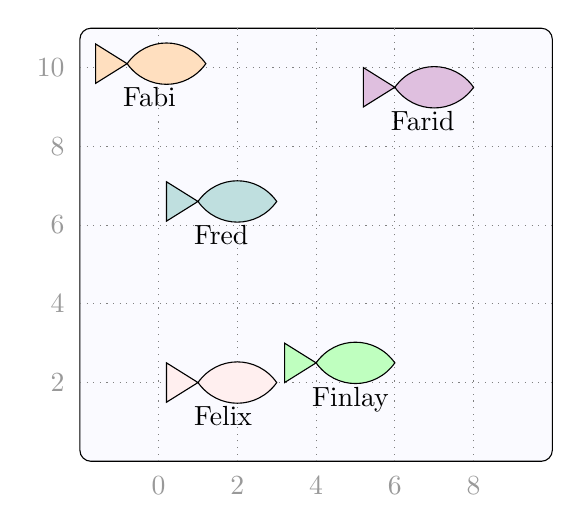
\begin{tikzpicture}[scale=0.5]
\draw[fill=blue!2, rounded corners] (-2,0) rectangle (10,11);
 % vertical dotted lines + x labels
  \foreach \x in {0,2,4,6,8} {
    \draw[dotted,gray] (\x,0) -- (\x,11);
    \node[below=2pt] at (\x,0) {\textcolor{black!40}{\x}};
  }

  % horizontal dotted lines + y labels
  \foreach \y in {2,4,6,8,10} {
    \draw[dotted,gray] (-2,\y) -- (10,\y);
    \node[left=2pt] at (-2,\y) {\textcolor{black!40}{\y}};
  }

\node[draw,shape=fish,fill=teal!25,align=center](fred) at (2,6.6) {Fred};
\node[draw,shape=fish,fill=orange!25](fabi) at (0.2,10.1) {Fabi};
\node[draw,shape=fish,fill=violet!25](farid) at (7,9.5) {Farid};
\node[draw,shape=fish,fill=pink!25](felix) at (2,2) {Felix};
\node[draw,shape=fish,fill=green!25](finlay) at (5,2.5) {Finlay};
\end{tikzpicture}
\end{center}
Your goal is to return the distance between the closest pair of fish.  In the example above, Felix and Finlay are closest, at distance $\sqrt{ (5-2)^2 + (2.5 - 2)^2 } = 3.04$ feet, so on input $F$, your algorithm should return $3.04$.

\textbf{Note:} The fact that the fish have names is not important for solving this problem, we just included them to make the example more clear.  If you like, you can assume that $F$ is an array of coordinate pairs $(x,y)$ with no names, rather than an array of triples $($name, $x,y)$.  If you drop the names, state so clearly in your solution.

\begin{enumerate}
\item \pts{5}
Design a divide-and-conquer algorithm that determines whether there exists a pair of fish within 1 foot of each other, on an input list $F$ with $n$ fish.  Your algorithm should run in time $O(n \log n)$.  You may assume that $n$ is a power of two if you like.

\hint{Depending on how you do the problem, the following may eventually be helpful: Suppose that you have a bunch of fish, all of distance at least $d$ from each other.  Then at most $8$ of these fish can be contained in any $2d \times d$ rectangle.  (You can take this as a fact, but it might be fun to convince yourself of this).} 

\expecting{Pseudocode and a clear English description of what it is doing.  You do not need to prove correctness or justify the running time (yet).  You may use any algorithm we have seen in class as a black box.}

\item \pts{4}
Design a divide-and-conquer algorithm that returns the distance between the closest pair of fish, on an input list $F$ with $n$ fish.  Your algorithm should run in time $O(n \log n)$.  You may assume that $n$ is a power of two if you like.

\hint{We do not expect that it will be useful to use your solution from part (a) as a black box, but we do expect that similar ideas will be helpful for this part.} 

\expecting{Pseudocode and a clear English description of what it is doing. Your response should be self-contained, meaning that it should not only state what is different than your part (a) solution, the whole pseudocode should be in this part. You do not need to prove correctness or justify the running time (yet).  You may use any algorithm we have seen in class as a black box.}


\item \pts{4} Explain why your algorithm in part (b) is correct.  You don't need to give a formal proof, but your explanation should be convincing to the grader.  

\expecting{A clear explanation.  If you don't think that your algorithm is correct, you can say what's wrong for partial credit.}


\item \pts{4} Explain why the running time of your algorithm in part (b) is $O(n \log n)$.   

\expecting{A short explanation.  Writing down a recurrence relation, explaining why it is relevant, and explaining why it has the desired solution is sufficient.  
 If you don't think that the running time of your algorithm is $O(n \log n)$, say what you think the running time is and justify that instead for partial credit on this part.}

\end{enumerate}

\ifdefined\template
\begin{shaded}
\textbf{SOLUTION:}
\ifdefined\sol
\input{solutions/fishFriends.tex}
\fi
\end{shaded}
\fi






\end{enumerate}

\end{document}
